\documentclass[../../../../main.tex]{subfiles}

\begin{document}

\section*{第1問}

［解］$t = \log_a b$ とおくと，与方程式は
\[
x^2 - 2tx + \frac{1}{t} = 0 \quad \dots \text{①}
\]
となる。この2解は，$t^2 - \frac{1}{t} > 0 \iff t < 0, 1 < t \quad \dots \text{②}$ のもとで，
\[
x = t \pm \sqrt{t^2 - \frac{1}{t}}
\]
だから，題意から，
\[
0 < t - \sqrt{t^2 - \frac{1}{t}} < 1 < t + \sqrt{t^2 - \frac{1}{t}} \quad \dots \text{③}
\]
$t < 0$ の時，左側の不等式が成立せず，不適だから ②から，$1 < t$ である。この時，
\begin{align*}
③ &\iff t - 1 < \sqrt{t^2 - \frac{1}{t}} < t \quad (\because 1 - t < 0) \\
&\iff t^2 - 2t + 1 < t^2 - \frac{1}{t} < t^2 \quad (\text{各辺正}) \\
&\iff 1 < t \quad (\because 1 < t)
\end{align*}
となる。以上から，$1 < t$ であるから，
\[
1 < \log_a b
\]
だから，
\[
1 < a < b \quad \text{or} \quad b < a < 1
\]
である。

\newpage

\section*{第2問}

［解］$\mathrm{PQ} \mathbin{/\!/} \mathrm{BC}$ より，$\angle \mathrm{BQP} = \frac{\pi}{4}$ だから，
\[
\cos \angle \mathrm{AQR} = \frac{1}{\sqrt{2}} \cdot \frac{1}{\sqrt{2}} = \frac{1}{2} \quad \therefore \angle \mathrm{AQR} = \frac{\pi}{3} \quad \left(0 < \angle \mathrm{AQR} < \pi\right)
\]
従って，$\angle \mathrm{BRQ} = \angle \mathrm{CRS}$ より $\triangle \mathrm{CSR} \mathbin{\sim} \triangle \mathrm{BQR}$ なので，
\[
\angle \mathrm{ASR} = \angle \mathrm{AQR} = \frac{\pi}{3}
\]
となり，最後の条件から $\angle \mathrm{CST} = \frac{5}{6}\pi$ となる。図は下図。

\begin{center}
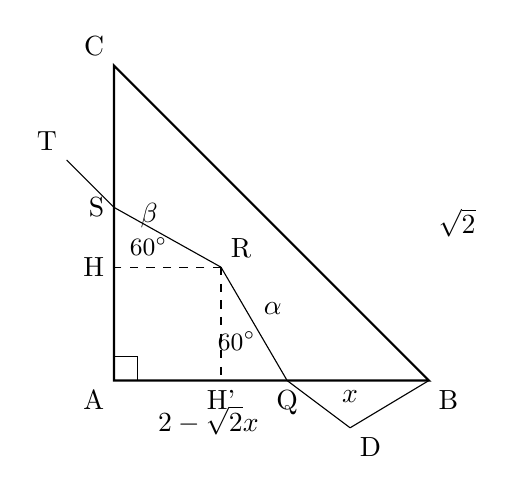
\begin{tikzpicture}[scale=2, >=stealth]
  % Triangle ABC
  \coordinate (A) at (0,0);
  \coordinate (B) at (2,0);
  \coordinate (C) at (0,2);

  \draw[thick] (A) -- (B) -- (C) -- cycle;
  \node[below left] at (A) {A};
  \node[below right] at (B) {B};
  \node[above left] at (C) {C};

  % Right angle mark at A
  \draw (0,0.15) -- (0.15,0.15) -- (0.15,0);

  % Points Q on AB, S on AC, R inside
  \coordinate (Q) at (1.1, 0);
  \coordinate (S) at (0, 1.1);
  \coordinate (R) at (0.68, 0.72);
  \coordinate (H) at (0, 0.72);
  \coordinate (Hp) at (0.68, 0);
  \coordinate (T) at (-0.3, 1.4);
  \coordinate (D) at (1.5, -0.3);

  \draw (R) -- (Q);
  \draw (R) -- (S);
  \draw[dashed] (R) -- (H);
  \draw[dashed] (R) -- (Hp);
  \draw (S) -- (T);
  \draw (B) -- (D);
  \draw (Q) -- (D);

  \node[below] at (Q) {Q};
  \node[left] at (S) {S};
  \node[above right] at (R) {R};
  \node[left] at (H) {H};
  \node[below] at (Hp) {H'};
  \node[above left] at (T) {T};
  \node[below right] at (D) {D};

  % Angles
  \node at (0.78, 0.25) {\small $60^\circ$};
  \node at (0.22, 0.85) {\small $60^\circ$};

  % Labels
  \node[above right] at (0.89, 0.36) {$\alpha$};
  \node[above left] at (0.34, 0.91) {$\beta$};
  \node[below] at (1.5, 0) {$x$};
  \node[right] at (2.0, 1.0) {$\sqrt{2}$};
  \node[below] at (0.6, -0.1) {$2-\sqrt{2}x$};
\end{tikzpicture}
\end{center}

$\mathrm{R}$ から $\mathrm{AC}, \mathrm{AB}$ に下ろした垂足を $\mathrm{H}, \mathrm{H'}$ とおき，$\overline{\mathrm{RQ}} = \alpha, \overline{\mathrm{SR}} = \beta$ とおく。$\overline{\mathrm{AB}} = 2$ だから，
\[
\begin{cases}
\mathrm{H'Q} = \frac{1}{2}\alpha, & \mathrm{RH'} = \mathrm{H'B} = \frac{\sqrt{3}}{2}\alpha \\[1ex]
\mathrm{HR} = \frac{\sqrt{3}}{2}\beta, & \mathrm{HS} = \frac{1}{2}\beta
\end{cases}
\]
\[
\therefore \begin{cases}
2 - \sqrt{2}x = \frac{1}{2}\alpha + \frac{\sqrt{3}}{2}\beta & \dots \text{①} \\[1ex]
2 - \sqrt{2}y = \frac{\sqrt{3}}{2}\alpha + \frac{1}{2}\beta & \dots \text{②} \\[1ex]
\frac{\sqrt{3}}{2}\alpha + \frac{\sqrt{3}}{2}\beta = 2 & \dots \text{③}
\end{cases}
\]
③より，$\alpha + \beta = \frac{4}{\sqrt{3}} = \frac{4}{3}\sqrt{3}$ だから，①+②に代入して求める関係式は
\begin{align*}
4 - \sqrt{2}x - \sqrt{2}y &= \left( \frac{\sqrt{3}}{2} + \frac{1}{2} \right) \cdot \frac{4}{3}\sqrt{3} \\
\therefore x + y &= \frac{1}{\sqrt{2}} \left\{ 4 - \frac{2}{3}(3+\sqrt{3}) \right\} \\
x + y &= \sqrt{2}\left( 1 - \frac{\sqrt{3}}{3} \right) \quad (x, y > 0)
\end{align*}

\bigskip

［＊以降］$\mathrm{A}$ を原点とし，$\mathrm{AB}$ を $x$ 軸とする座標を設定すると
\begin{align*}
\mathrm{RQ} &: y = -\sqrt{3}(x - A) \quad (A = 2 - \sqrt{2}x) \\
\mathrm{RS} &: y = -\frac{1}{\sqrt{3}}x + B \quad (B = 2 - \sqrt{2}y)
\end{align*}
この交点 $\left( \frac{3A - \sqrt{3}B}{2}, \frac{-\sqrt{3}A + 3B}{2} \right)$ が $x + y = 2$ 上にあることが必要十分．
\[
\frac{3A - \sqrt{3}B}{2} + \frac{-\sqrt{3}A + 3B}{2} = 2
\]
\[
(3 - \sqrt{3})(A + B) = 4
\]
\[
\therefore x + y = \sqrt{2} \left( 1 - \frac{\sqrt{3}}{3} \right)
\]

\newpage

\section*{第3問}

［解］右図のように $xy$ 平面をとる。

$|\mathrm{OA}| = 1, |\mathrm{AB}| = 1$ としても良い。$\mathrm{A}$ から $g$ に下ろした垂足を $\mathrm{H}$ とする。又，$G$ が最低の時を考えるので $\mathrm{A}$ は $g$ の下側にあるとして良い。

$\angle \mathrm{BOA} = \beta$ とおく。$|\mathrm{AB}| = |\mathrm{OA}|$ から $H$ は $\mathrm{OB}$ の中点である。

\begin{center}
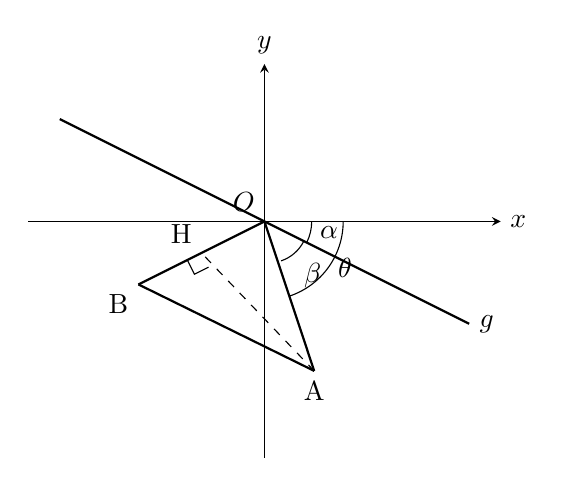
\begin{tikzpicture}[scale=2, >=stealth]
  % Axes
  \draw[->] (-1.5, 0) -- (1.5, 0) node[right] {$x$};
  \draw[->] (0, -1.5) -- (0, 1.0) node[above] {$y$};
  \node[above left] at (0,0) {$O$};

  % Line g at angle -alpha
  \draw[thick] (-1.3, 0.65) -- (1.3, -0.65) node[right] {$g$};
  
  % Point A at angle -theta
  \coordinate (A) at (0.316, -0.949);
  \coordinate (B) at (-0.8, -0.4);
  \coordinate (H) at (-0.4, -0.2);

  \draw[thick] (0,0) -- (A) node[below] {A};
  \draw[thick] (0,0) -- (B) node[below left] {B};
  \draw[thick] (B) -- (A);
  \draw[dashed] (A) -- (H) node[above left] {H};

  % Angle arcs
  \draw (0.3, 0) arc (0:-26.57:0.3) node[midway, right] {$\alpha$};
  \draw (0.5, 0) arc (0:-71.57:0.5) node[midway, right] {$\theta$};
  \draw (0.25, -0.125) arc (-26.57:-71.57:0.25) node[midway, below right] {$\beta$};

  % Right angle mark at H
  \draw (-0.355, -0.29) -- (-0.445, -0.335) -- (-0.49, -0.245);
\end{tikzpicture}
\hfil
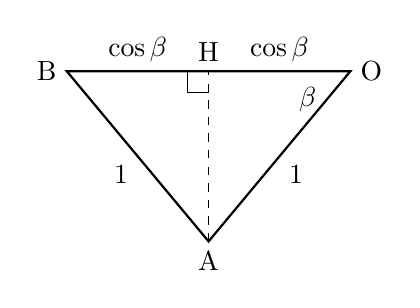
\begin{tikzpicture}[scale=1.8, >=stealth]
  % Isosceles triangle OAB with altitude AH
  \coordinate (O) at (0,0);
  \coordinate (B) at (2,0);
  \coordinate (H) at (1,0);
  \coordinate (A) at (1,-1.2);

  \draw[thick] (O) node[left] {B} -- (B) node[right] {O} -- (A) node[below] {A} -- cycle;
  \draw[dashed] (A) -- (H) node[above] {H};
  
  % Right angle mark
  \draw (0.85, 0) -- (0.85, -0.15) -- (1, -0.15);

  \node[above] at (0.5, 0) {$\cos\beta$};
  \node[above] at (1.5, 0) {$\cos\beta$};
  \node[below left] at (0.5, -0.6) {1};
  \node[below right] at (1.5, -0.6) {1};
  \node at (1.7, -0.2) {$\beta$};
\end{tikzpicture}
\end{center}

\begin{align*}
\mathrm{A}&(\cos(-\theta), \sin(-\theta)) \\
\mathrm{H}&(\cos\beta \cos(-\alpha), \cos\beta \sin(-\alpha))
\end{align*}
だから，
\begin{align*}
\vec{\mathrm{OG}} &= \vec{\mathrm{OH}} + \frac{1}{2}\vec{\mathrm{HA}} = \frac{1}{2}\vec{\mathrm{OH}} + \frac{1}{2}\vec{\mathrm{OA}} \\
&= \frac{1}{2} \cos\beta \begin{pmatrix} \cos\alpha \\ -\sin\alpha \end{pmatrix} + \frac{1}{2} \begin{pmatrix} \cos\theta \\ -\sin\theta \end{pmatrix}
\end{align*}
である。この $y$ 座標を $Y$ として
\[
Y = -\frac{1}{2} [ \sin\alpha \cos\beta + \sin\theta ]
\]
これが最小になる時の $\tan\theta$ をもとめれば良い。$\alpha + \beta = \theta$ から，
\begin{align*}
Y &= -\frac{1}{2} \left[ \frac{1}{2}(\sin(\alpha+\beta) + \sin(\alpha-\beta)) + \sin\theta \right] \\
&= -\frac{1}{2} \left[ \frac{3}{2}\sin\theta + \frac{1}{2}\sin(2\alpha-\theta) \right] \quad \dots \text{①}
\end{align*}
$\tan\alpha = \frac{1}{2}$ より，($0 < \alpha < \pi/2$ とあわせて)
\[
\begin{cases}
\sin 2\alpha = \frac{2 \cdot \frac{1}{2}}{1 + (\frac{1}{2})^2} = \frac{4}{5} \\[1ex]
\cos 2\alpha = \frac{1 - (\frac{1}{2})^2}{1 + (\frac{1}{2})^2} = \frac{3}{5}
\end{cases}
\]
だから ①に代入して，以下 $S = \sin\theta, C = \cos\theta$ として，
\begin{align*}
Y &= -\frac{1}{4} \left[ 3S + \frac{4}{5}C - \frac{3}{5}S \right] \\
&= -\left( \frac{3}{5}S + \frac{1}{5}C \right) \\
&\ge -\sqrt{\left(\frac{3}{5}\right)^2 + \left(\frac{1}{5}\right)^2} \quad (\because \text{コーシー・シュワルツ})
\end{align*}
等号成立は $\begin{pmatrix} 3/5 \\ 1/5 \end{pmatrix} \mathbin{/\!/} \begin{pmatrix} S \\ C \end{pmatrix}$ の時で，この時
\[
\frac{1}{5}S - \frac{3}{5}C = 0
\]
\[
\therefore \tan\theta = \frac{S}{C} = 3
\]
となる。

\newpage

\section*{第4問}

［解］$S_n = \sum_{k=1}^n \frac{r^{2^{k-1}}}{1 - r^{2^k}}$ とおく。
\[
S_n = \sum_{k=1}^n \left( \frac{1}{1 - r^{2^{k-1}}} - \frac{1}{1 - r^{2^k}} \right) = \frac{1}{1-r} - \frac{1}{1 - r^{2^n}} \quad \dots \text{①}
\]
だから，
\[
\begin{cases}
|r| > 1 \text{ の時} & S_n \to \frac{1}{1-r} \\[1.5ex]
|r| < 1 \text{ の時} & S_n \to \frac{1}{1-r} - 1 = \frac{r}{1-r}
\end{cases}
\]
となる。

\end{document}
